%************************************************
\chapter{DUMMY vorlagen}\label{ch:vorlagen}
%************************************************

Qellentest:


inBin\cite[12]{inBin} hauptref \cite[1.4]{perfAv} GreenOrbs \cite[Kap. 3]{GreenOrbs} X-Mac\cite{xmac} Model\cite{model} Stanard\cite{ieee} Datenblatt\cite{CC1200data} User Guide\cite{CC1200guide}


\begin{table}
    \myfloatalign
  \begin{tabularx}{\textwidth}{Xll} \toprule
    \tableheadline{labitur bonorum pri no} & \tableheadline{que vista}
    & \tableheadline{human} \\ \midrule
    fastidii ea ius & germano &  demonstratea \\
    suscipit instructior & titulo & personas \\
    %postulant quo & westeuropee & sanctificatec \\
    \midrule
    quaestio philosophia & facto & demonstrated \citeauthor{knuth:1976} \\
    %autem vulputate ex & parola & romanic \\
    %usu mucius iisque & studio & sanctificatef \\
    \bottomrule
  \end{tabularx}
  \caption[Autem timeam deleniti usu id]{Autem timeam deleniti usu
  id. \citeauthor{knuth:1976}}  \label{tab:example}
\end{table}

nalsndlkasndlaksndlaskndlaksndlaksndlaksnd lskjf lslkdf lslkdfm llslkdmf lslkmdf lkmsd flsldkfm lsmdf lsldkf llsldkfm lsldkfm  lsf lslsdkfm lslkdmf lsldkf lsdkf llsldkmf lsldf äfqäwejflkf älskdf  öasdkfm ls aälsk lsldkf wlefweor lksdf lkem lsl l sldfm sll lsdm lmmld lskd lslsldkfm lllsdfm lslldfk llk lslsdkf lsldfl lslskfm lsslkf lsldkf llsldkf llskdfm lslölskdf lsldkmf llsldfk lsdfmlsdkmfaldkfmöalksdf llsdlslefsldf lsdflef 

\begin{figure}[bth]
        \myfloatalign
        \subfloat[Asia personas duo.]
        {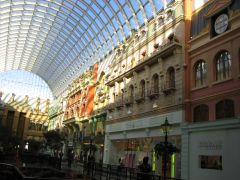
\includegraphics[width=.45\linewidth]{gfx/example_1}} \quad
        \subfloat[Pan ma signo.]
        {\label{fig:example-b}%
         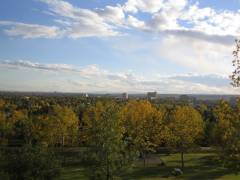
\includegraphics[width=.45\linewidth]{gfx/example_2}} \\
        \subfloat[Methodicamente o uno.]
        {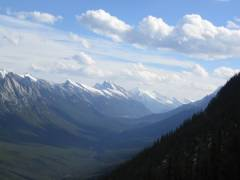
\includegraphics[width=.45\linewidth]{gfx/example_3}} \quad
        \subfloat[Titulo debitas.]
        {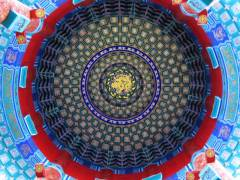
\includegraphics[width=.45\linewidth]{gfx/example_4}}
        \caption[Tu duo titulo debitas latente]{Tu duo titulo debitas
        latente. }\label{fig:example}
\end{figure}
alskdlaksmdlasmdlasmdlasmdlaskmd

\begin{lstlisting}[float=b,language=Pascal,frame=tb,caption={A floating example (\texttt{listings} manual)},label=lst:useless]
for i:=maxint downto 0 do
begin
{ do nothing }
end;
\end{lstlisting}

alskdjlaksd ölaskdölaks dmföalksdm fölaksdmfösalk  dmföaskldfmöalskmd  föaksdmfösak mdföak msdöfka msdöfkam sö dfkm öasldf möas kldm föskdmfasdfsad
sdfalskdföa skdnfö lksadn öflksd nfölksd   nöflksndöflkasndölfka nsön dfasnödkfsad fsd  
söldkföaslkdnfölaskdnfölkasdnfölkasndöfl  knasödlk  föslkdfn lskdfnslkdnflsk dnfksdlfka nsld kfnlaksnd  flkasndflksnd lfknslkdnfl aks  dnflka sndflksdnlf ksndlfknsldf knklalalkasd  lkmsl dkm alksmdlaksm  dlaksmdlaksm daskdmalskd malskdmalskds

\begin{equation}
\kappa =\frac{\xi}{E_{\textrm{max}}} %\mathbb{ZNR}
\end{equation}
$E_{\textrm{max}}$ is the maximum transferable energy in a single
collision with an atomic electron.

$\xi$ comes from the Rutherford scattering cross section
and is defined as:
\begin{eqnarray*} \xi  = \frac{2\pi z^2 e^4 N_{\textrm{Av}} Z \rho
\delta x}{m_{\textrm{e}} \beta^2 c^2 A} =  153.4 \frac{z^2}{\beta^2}
\frac{Z}{A}
  \rho \delta x \quad\textrm{keV},
\end{eqnarray*}
where

\begin{tabular}{ll}
$z$          & charge of the incident particle \\
$N_{\textrm{Av}}$     & Avogadro's number \\
$Z$          & atomic number of the material \\
$A$          & atomic weight of the material \\
$\rho$       & density \\
$ \delta x$  & thickness of the material \\
\end{tabular}

$\kappa$ measures the contribution of the collisions with energy

lskdlksdlsdlkasldkalsdkalskdasd

%*****************************************
%*****************************************
%*****************************************
%*****************************************
%*****************************************




